\let\negmedspace\undefined
\let\negthickspace\undefined
\documentclass[journal]{IEEEtran}
\usepackage[a5paper, margin=10mm, onecolumn]{geometry}
%\usepackage{lmodern} % Uncomment if needed for pdflatex
\usepackage{tfrupee} % Include tfrupee package

\setlength{\headheight}{1cm} % Set the height of the header box
\setlength{\headsep}{0mm}     % Set the distance between the header box and the top of the text

\usepackage{gvv-book}
\usepackage{gvv}
\usepackage{cite}
\usepackage{amsmath,amssymb,amsfonts,amsthm}
\usepackage{algorithmic}
\usepackage{graphicx}
\usepackage{textcomp}
\usepackage{xcolor}
\usepackage{txfonts}
\usepackage{listings}
\usepackage{enumitem}
\usepackage{mathtools}
\usepackage{gensymb}
\usepackage{comment}
\usepackage[breaklinks=true]{hyperref}
\usepackage{tkz-euclide} 
\usepackage{listings}
%\usepackage{gvv}                                        
\def\inputGnumericTable{}                                 
\usepackage[latin1]{inputenc}                                
\usepackage{color}                                            
\usepackage{array}                                            
\usepackage{longtable}                                       
\usepackage{calc}                                             
\usepackage{multirow}                                         
\usepackage{hhline}                                           
\usepackage{ifthen}                                           
\usepackage{lscape}
\usepackage{tikz}
\usepackage{circuitikz}
\usepackage{standalone} % For including external TikZ files

\begin{document}

\bibliographystyle{IEEEtran}
\vspace{3cm}

\title{8.1.3}
\author{EE24BTECH11066 - YERRA AKHILESH}
% \maketitle
% \newpage
% \bigskip
{\let\newpage\relax\maketitle}

\renewcommand{\thefigure}{\theenumi}
\renewcommand{\thetable}{\theenumi}
\setlength{\intextsep}{10pt} % Space between text and floats

\numberwithin{equation}{enumi}
\numberwithin{figure}{enumi}
\renewcommand{\thetable}{\theenumi}
\textbf{Question}:\\
Find the area of the region bounded by $x^2 = 4y, y = 2, y = 4$ and the y-axis in the first quadrant.\\
\textbf{Solution: }\\
\textbf{Theoritical Solution:}\\
Express $x$ in terms of $y$,
\begin{align}
    x = 2 \sqrt{y}\\
    (or) \\
    x = -2 \sqrt{y}
\end{align}
But we should take first equation as we have to find the area in the first quadrant,\\
Area under the curve is given by,
\begin{align}
    A = \int_{2}^{4} 2 \sqrt{y} \, dy\\
    A = 2 \brak{\frac{y^{\frac{3}{2}}}{\frac{3}{2}}} \Big|_2^4\\
    A = \frac{4}{3} \brak{4^{\frac{3}{2}} - 2^{\frac{3}{2}}}\\
    A = \frac{4}{3} \brak{8 - 2\sqrt{2}}\\
    A = 6.895
\end{align}
\textbf{Computational Solution:} 
Taking trapezoid-shaped strips of small area and adding them all up. Say we have to find the area of $y_{x}$ from $x = x_0$ to $x = x_n$, discretize the points on the $x$ axis $x_0, x_1, x_2, \dots, x_n$ such that they are equally spaced with the step size $h$. \\
Sum of all trapezoidal areas is given by,
\begin{align}
  A &= \frac{1}{2}h\brak{y\brak{x_1}+y\brak{x_0}}+ \frac{1}{2}h\brak{y\brak{x_2}+y\brak{x_1}}+\dots+\frac{1}{2}h\brak{y\brak{x_n}+y\brak{x_{n-1}}}\\
  &= h\sbrak{\frac{1}{2}\brak{y\brak{x_0}+y\brak{x_n}}+ y\brak{x_1}+\dots+y\brak{x_{n-1}}}
\end{align}
Let $A\brak{x_n}$ be the area enclosed by the curve $y\brak{x}$ from $x = x_0$ to $x = x_n$, $\brak{x_0, x_1, \dots x_n}$ be equidistant points with step-size $h$.
\begin{align}
  A\brak{x_n+h} = A\brak{x_n}+\frac{1}{2}h\brak{y\brak{x_n+h}+y\brak{x_n}}
\end{align}
We can repeat this till we get the required area.\\
Discretizing the steps, making $A\brak{x_n} = A_n, y\brak{x_n} = y_n$ we get,
\begin{align}
 A_{n+1} = A_n+\frac{1}{2}h\brak{y_{n+1}+y_n}
\end{align}
We can write $y_{n+1}$ in terms of $y_n$ using the first principle of derivative. $y_{n+1} = y_n + hy^{\prime}_n$
\begin{align}
  A_{n+1} &= A_n+\frac{1}{2}h\brak{\brak{y_{n}+hy^{\prime}_n}+y_n}\\
  A_{n+1} &= A_n+\frac{1}{2}h\brak{2y_n+hy^{\prime}_n}\\
  A_{n+1} &= A_n+hy_n+\frac{1}{2}h^2y^{\prime}_n\\
  x_{n+1} &= x_n+h
\end{align}
In the given question, $y_n = \frac{x_n^2}{4}$ and $y^{\prime}_n = \frac{x_n}{2}$. \\
The general difference equation will be given by
\begin{align}
  A_{n+1} &= A_n+hy_n+\frac{1}{2}h^2y^{\prime}_n\\
  A_{n+1} &= A_n+h\brak{\frac{x_n^2}{4}}+\frac{1}{2}h^2\brak{\frac{x_n}{2}}\\
  x_{n+1} &= x_n+h
\end{align}
Iterating till we reach $x_n = 4$ will return the required area. \\

Area obtained computationally: $6.895$ sq. units.\\

Area obtained theoretically: $\frac{4}{3} \brak{8 - 2\sqrt{2}}$ = 6.895 sq.units\\
\begin{figure}[ht!]
   \centering
   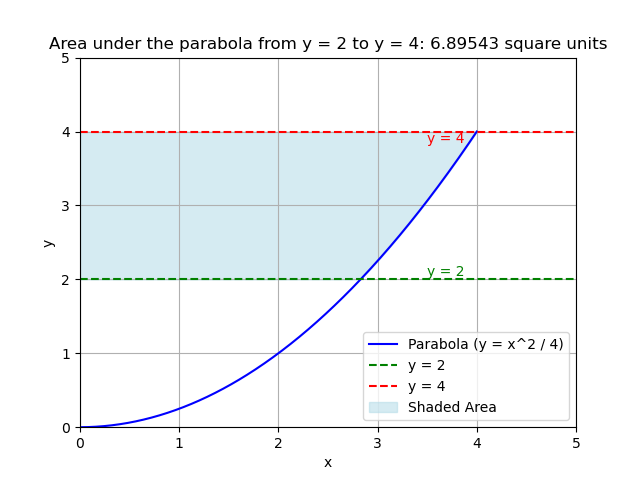
\includegraphics[width=\columnwidth]{figs/Figure_1.png}
\end{figure}
\end{document}
